\section{Clustering}\label{sec:results:clustering}
In gauging how effective our clustering method is against \cplop{}, we looked at the distribution of cluster sizes, the number of \isols{} that fell into high purity clusters, the number of unique species in each cluster and how that affected the size and purity, and overall coverage and accuracy metrics.
From these data, we gained some insight into the clustering algorithm and were able to visualize some predictions we had about the biological aspects of strains.  

% SIZES --------------------
\subsection{Cluster Size Distribution}
\begin{sidewaysfigure}
    \centering
    \subfloat[
        Cluster Size Distribution for \minneigh{} of 3
        ]{
        \label{fig:clust_size_dist_3}
        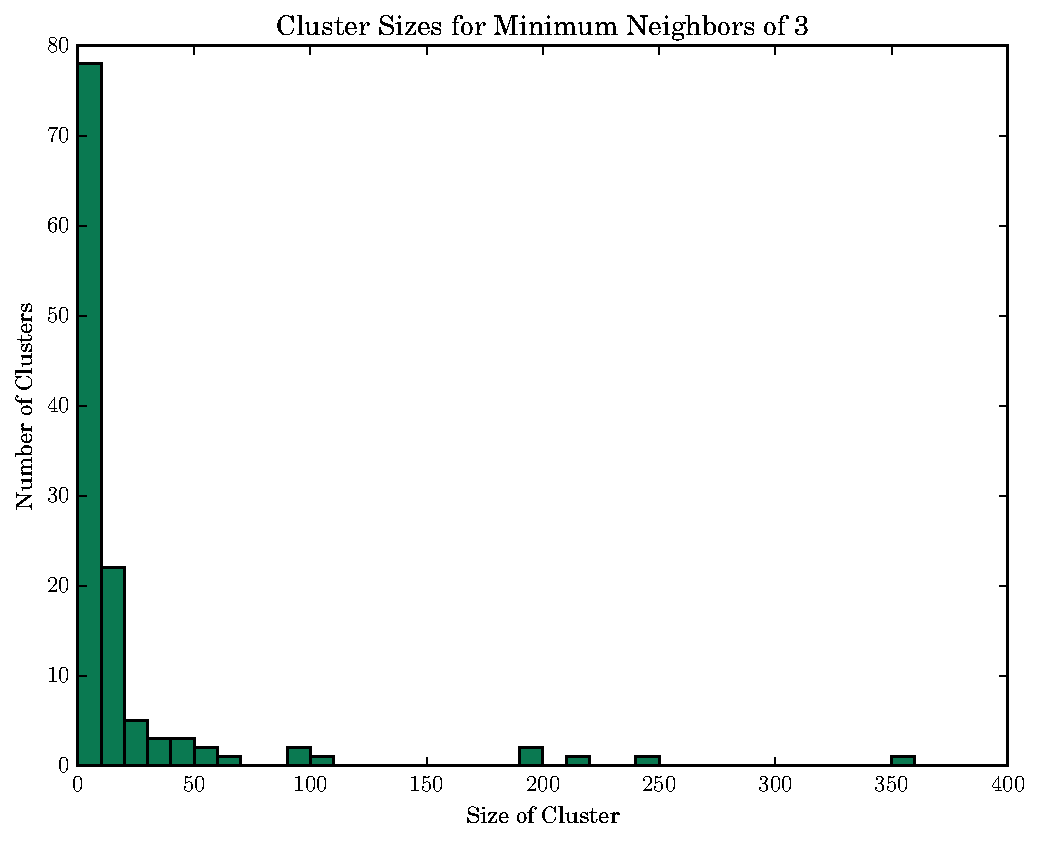
\includegraphics[width=0.30\linewidth]{figures/bs/neigh_size_3}
    }
    \hfill
    \subfloat[
        Cluster Size Distribution for \minneigh{} of 5
        ]{
        \label{fig:clust_size_dist_5}
        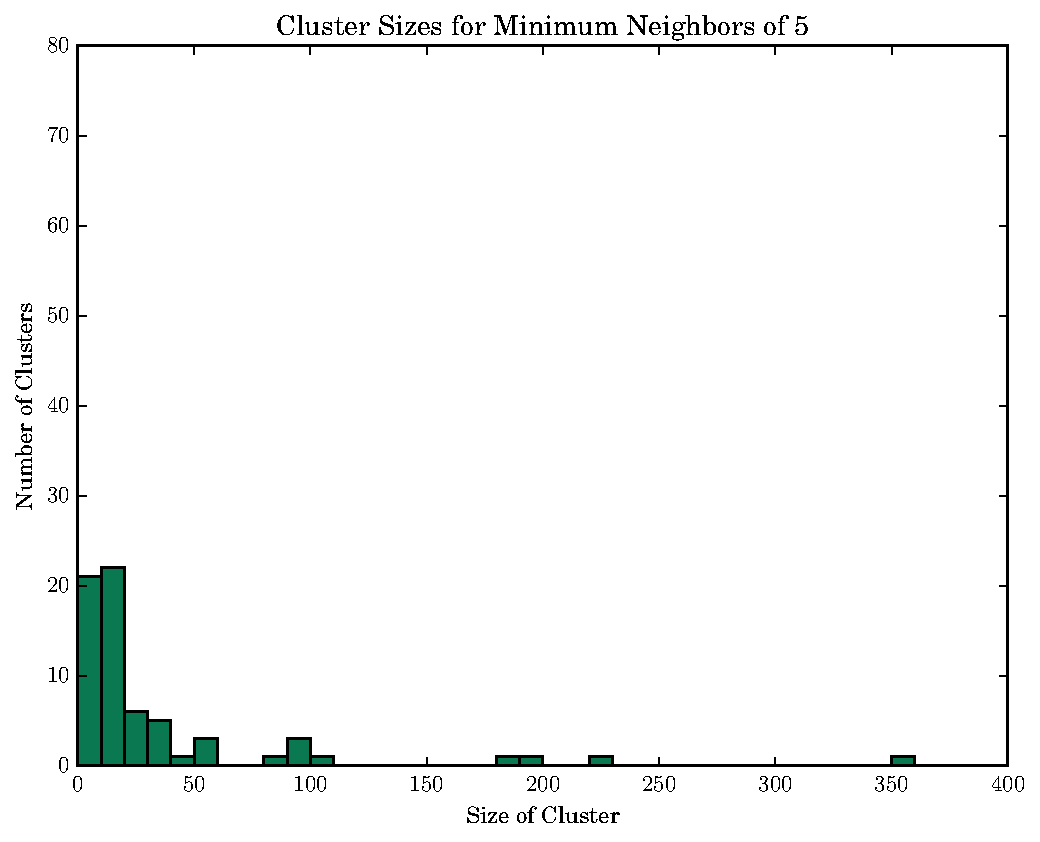
\includegraphics[width=0.30\linewidth]{figures/bs/neigh_size_5}
    }
    \hfill
    \subfloat[
        Cluster Size Distribution for \minneigh{} of 7
        ]{
        \label{fig:clust_size_dist_7}
        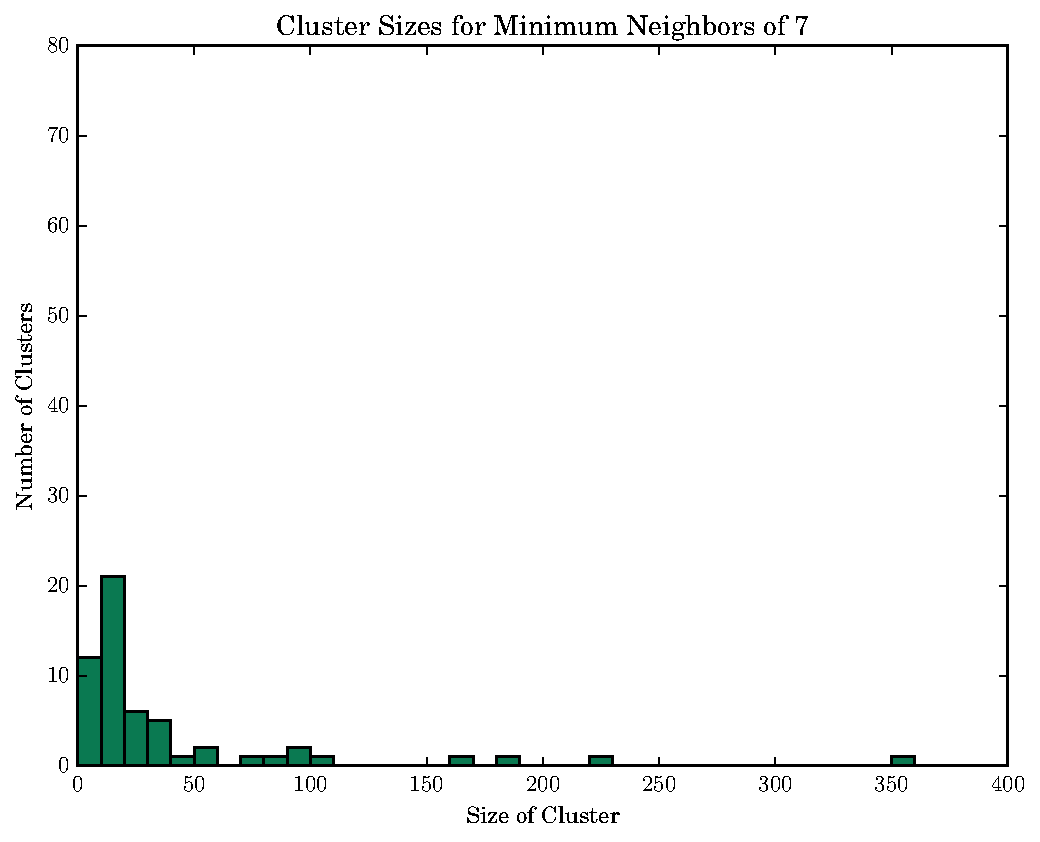
\includegraphics[width=0.30\linewidth]{figures/bs/neigh_size_7}
    }
    \caption{The size distribution of clusters skews heavily towards smaller clusters.}
    \label{fig:clust_size_dist}
\end{sidewaysfigure}

\autoref{fig:clust_size_dist} shows the distribution of cluster sizes as \minneigh{} increase from 3, to 5, to 7. 
We see that at all three \minneigh{} values, the number of small clusters (fewer than 10) dominates the overall makeup of clusters.
\autoref{fig:clust_size_dist} shows a propensity towards small clusters at low \minneigh{} values.
This creates a high number of 100\% or almost 100\% pure clusters.
Most clusters are tiny, with a few larger clusters for small \minneigh{} values.

As we approach higher \minneigh{} values, the smaller clusters disappear.
As \minneigh{} increases from 3 to 5, we lose over half of clusters of size smaller than 10; while as \minneigh{} increases to 7, we lose only a few more.
Furthermore, while the number of clusters with 10-20 \isols{} stays relatively stable across \minneigh{} values, the number of clusters with 50-100 \isols{} increase for \minneigh{} of 5 and 7.

% PURITIES --------------------
\subsection{Cluster Purity Distribution}
\begin{sidewaysfigure}
    \centering
    \subfloat[
        Cluster Purity Distribution for \minneigh{} of 3
        ]{
        \label{fig:clust_purity_dist_3}
        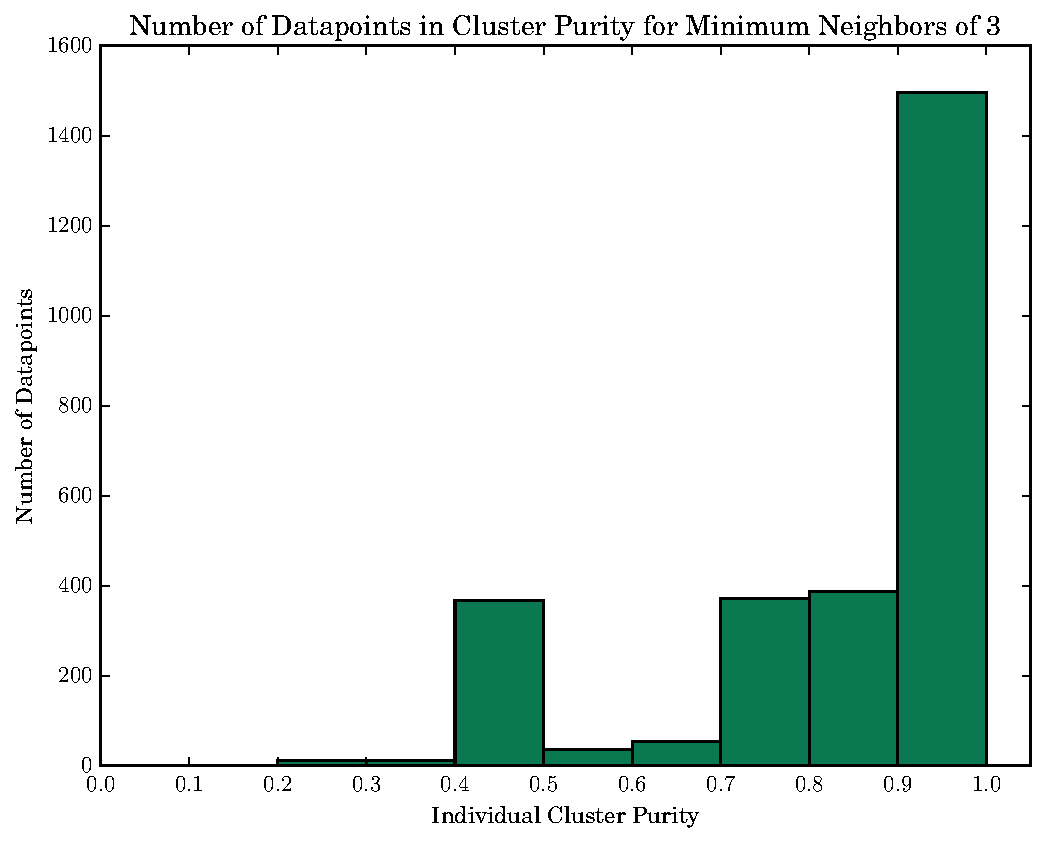
\includegraphics[width=0.30\linewidth]{figures/bs/neigh_dist_data_3}
    }
    \hfill
    \subfloat[
        Cluster Purity Distribution for \minneigh{} of 5
        ]{
        \label{fig:clust_purity_dist_5}
        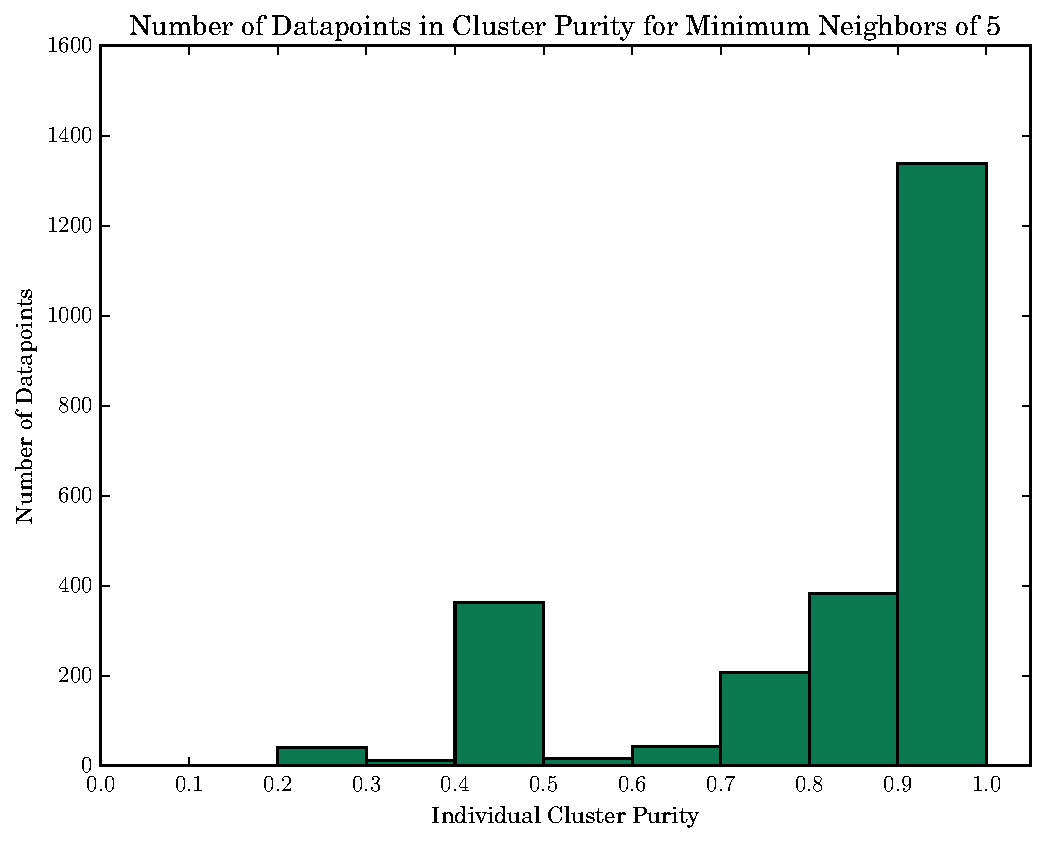
\includegraphics[width=0.30\linewidth]{figures/bs/neigh_dist_data_5}
    }
    \hfill
    \subfloat[
        Cluster Purity Distribution for \minneigh{} of 7
        ]{
        \label{fig:clust_purity_dist_7}
        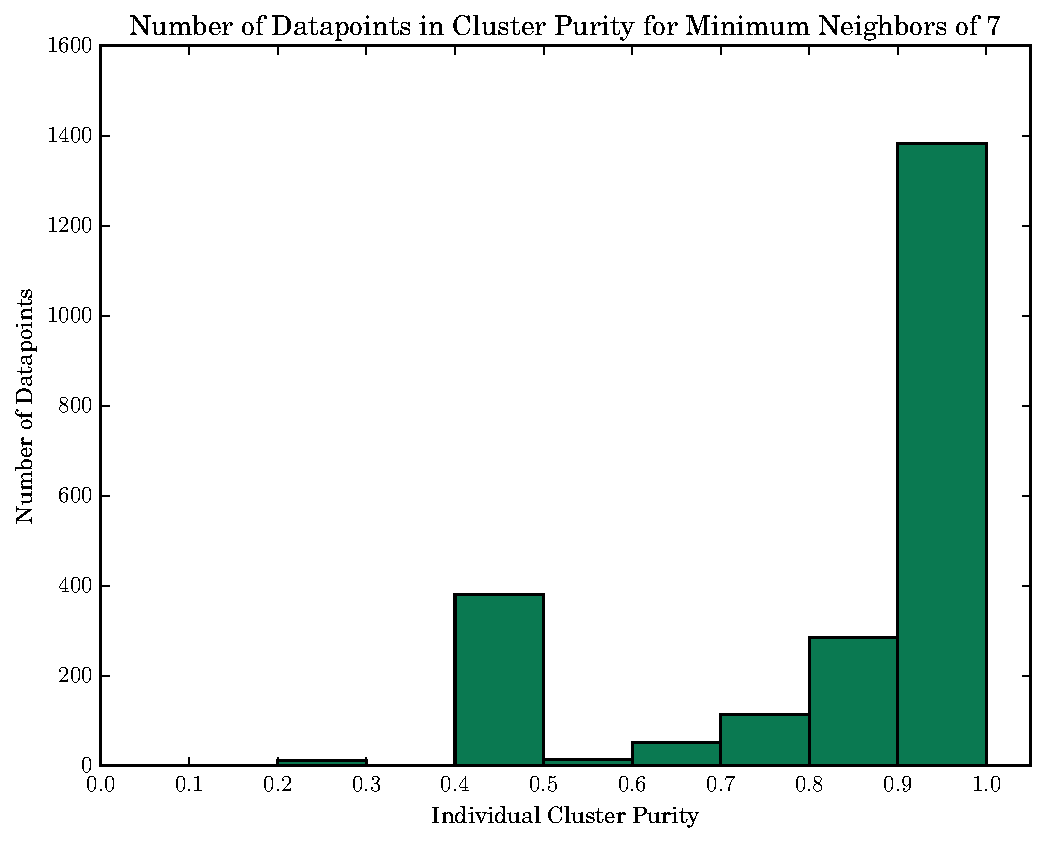
\includegraphics[width=0.30\linewidth]{figures/bs/neigh_dist_data_7}
    }
    
    \caption{The number of \isols{} that fall into a cluster of a given purity. We notice that that the number of \isols{} that fall into the 0.90 to 1.00 cluster purity range decreases as we increase \minneigh{} from 3 to 5, but increases from 5 to 7.}
    \label{fig:clust_purity_dist}
\end{sidewaysfigure}

Of interest to our investigation is the number of \isols{} that fall within clusters of a particular purity. 
\autoref{fig:clust_purity_dist} shows the number of \isols{} that fall within a cluster of a particular purity as a histogram.
We notice that as \minneigh{} increases, the purity skews towards purer clusters and that a portion of \isols{} remain in an impure cluster regardless of the \minneigh{} value.

From \minneigh{} of 3 all the way to 7, there are about 400 \isols{} that land in a cluster of purity between 0.4 and 0.5.  
This group of isolates remains largely unchanged as we restrict the \minneigh{} value.
We suspect (and discuss in \autoref{sec:results:discussion}) that certain \ecoli{} strains find themselves in many \spec{} fecal matter.

% UNIQUE --------------------
\subsection{Unique Species in Each Cluster}\label{sec:results:unique}

\begin{sidewaysfigure}
    \centering
    \subfloat[
        Cluster Purity for \minneigh{} of 3
        ]{
        \label{fig:clust_pure_3}
        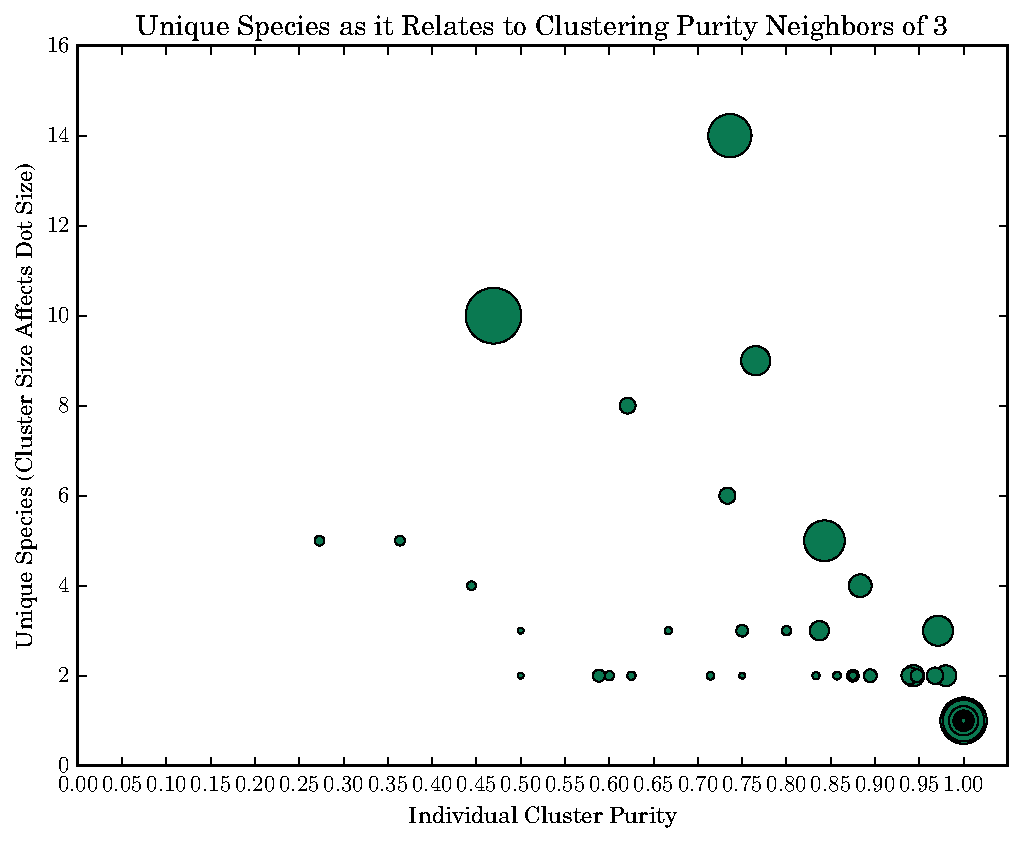
\includegraphics[width=0.30\linewidth]{figures/bs/neigh_purity_unique_3_size}
    }
    \hfill
    \subfloat[
        Cluster Purity for \minneigh{} of 5
        ]{
        \label{fig:clust_pure_5}
        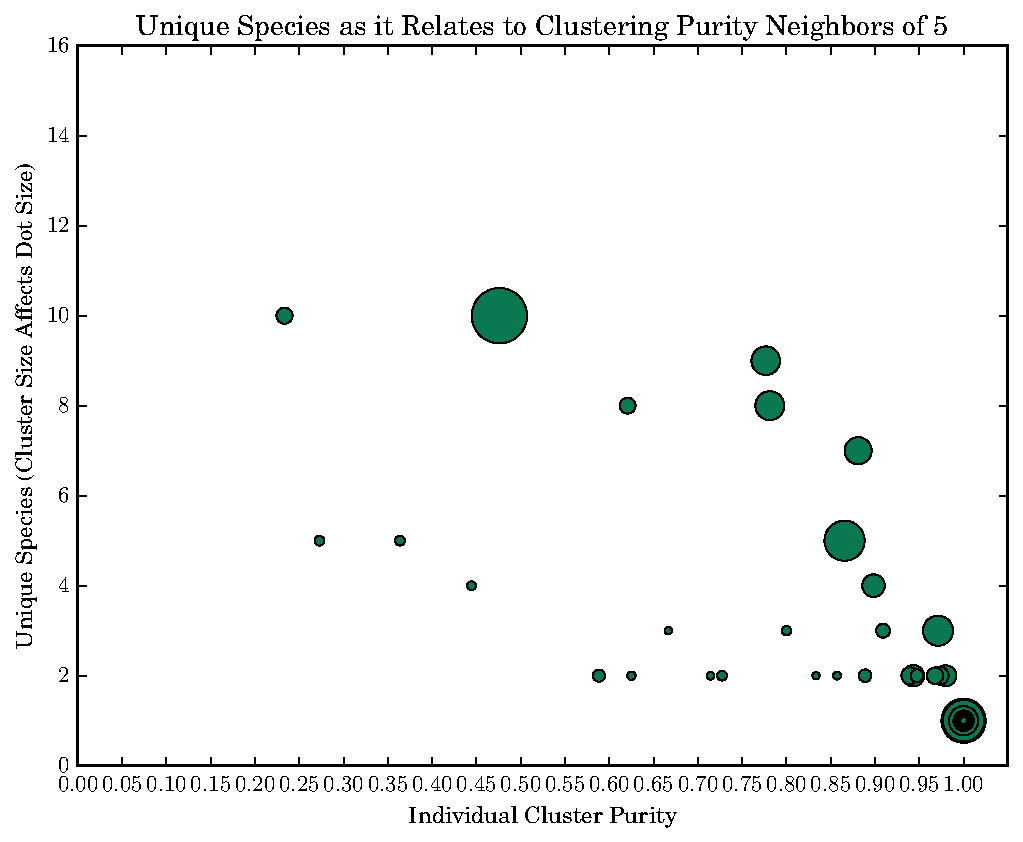
\includegraphics[width=0.30\linewidth]{figures/bs/neigh_purity_unique_5_size}
    }
    \hfill
    \subfloat[
        Cluster Purity for \minneigh{} of 7
        ]{
        \label{fig:clust_pure_7}
        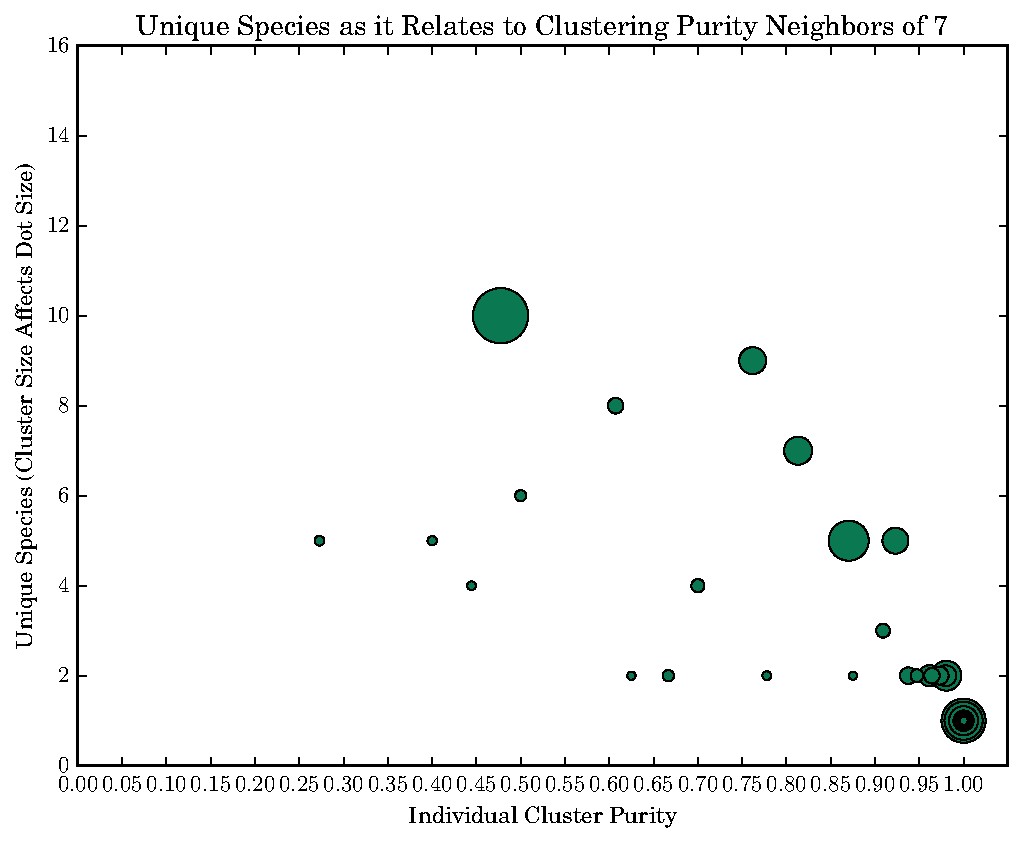
\includegraphics[width=0.30\linewidth]{figures/bs/neigh_purity_unique_7_size}
    }

    \caption{These three dimensional graphs show the individual cluster purity in the horizontal axis, the number of unique species in the vertical axis, and the relative size of the cluster in the diameter of the dots. Each individual dot is its own cluster. We find that as we restrict cluster to needing more neighbors (increasing the \minneigh{} value), we lose some clusters and gain more pure clusters.}
    \label{fig:clust_pure}
\end{sidewaysfigure}

Knowing the number of unique \spec{} in our clusters is key to understanding how our
strain-based \mst{} algorithm  performs.
\autoref{fig:clust_pure} plots the number of unique species in each cluster (vertical axis) against
individual cluster purity (horizontal axis) representing each cluster as a circle of diameter
proportional to cluster size\footnote{A linear scaling of the diameter with respect to \textit{the largest cluster amongst all the clusterings} defines the diameters of the dots.}.
The points at the lower right represent many clusters of various size of 100\% (or near so) purity and are stacked from largest behind cluster to smallest in front.

As \minneigh{} values increase  we see one cluster at the top right
(\minneigh{}=3) with 14 unique species disappear  as \minneigh{} becomes $5$.
One very low purity cluster at a \minneigh{} value of 5 disappears 
when we increase \minneigh{} to 7 in \autoref{fig:clust_pure_7}.

A particularly large cluster at around 0.45 purity with 11 unique \spec{}, remains relatively intact
(and is clearly recognizable)
as \minneigh{} changes from 3, to 5, to 7. 
This can account for the large amount of \isols{} clustered into impure clusters in \autoref{fig:clust_purity_dist}.

As we restrict the cluster size with \minneigh{}, we see that this appears to break up some clusters and cause others to become bigger.
It is difficult to track exactly how a cluster changes without making some simplifying assumptions or without tracking all 4,610 \isols{} as they move from cluster to cluster.

% COVERAGE --------------------
\subsection{Clustering Coverage}
\begin{figure}[ht!]
    \centering
    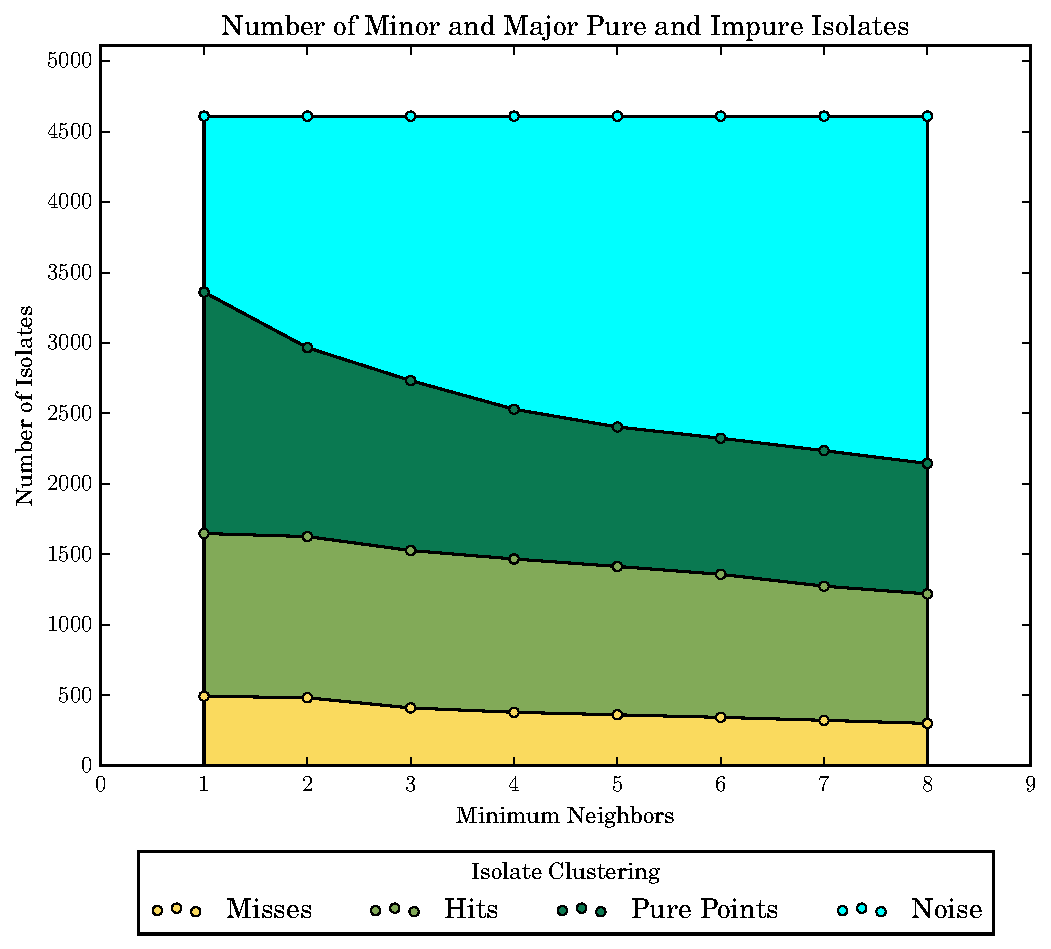
\includegraphics[width=\linewidth]{figures/bs/neigh_minor_major_impure_filled_stack}
    \caption{As \minneigh{} increases, we see that we cluster fewer \isols{}. throughout, the number of major pure \isols{} stays relatively equal to the number of major impure \isols{}.}
    \label{fig:clustered}
\end{figure}

Clustering coverage is important to consider, since we want our clustering algorithm to apply to as many \isols{} as possible.
Towards this end we investigated the four metrics introduced in \autoref{sec:validation:coverage} --- noise, misses, hits, and pure points --- for each \minneigh{} clustering investigated.
We hope to find the \minneigh{} value that gives us the most pure points, but will also settle for the fewest misses, shown in \autoref{fig:clustered}.

The cyan area is noise --- \isols{} that were not clustered. 
The dark green area is the proportion of pure points. 
Light green is the number of hits.
Gold is the number of misses.

It is good to note that the number of misses are low and flatten out as we increase \minneigh{} from a value of 3, giving us good reason not to investigate clustering where \minneigh{} is greater than we have already investigated.
The number of pure points stays relatively equal to the number of hits.
Important in \autoref{fig:clustered} is the amount of \isols{} that the algorithm does cluster.
The combination of the gold and two green areas show the total number clustered, while the cyan shows the number of \isols{} that were \textit{not} clustered.
It is unfortunate that the number of noise \isols{} is high, but we plan to mitigate that in future work.

% OVERALL --------------------
\subsection{Overall Clustering Purity}
\begin{figure}[ht!]
    \centering
    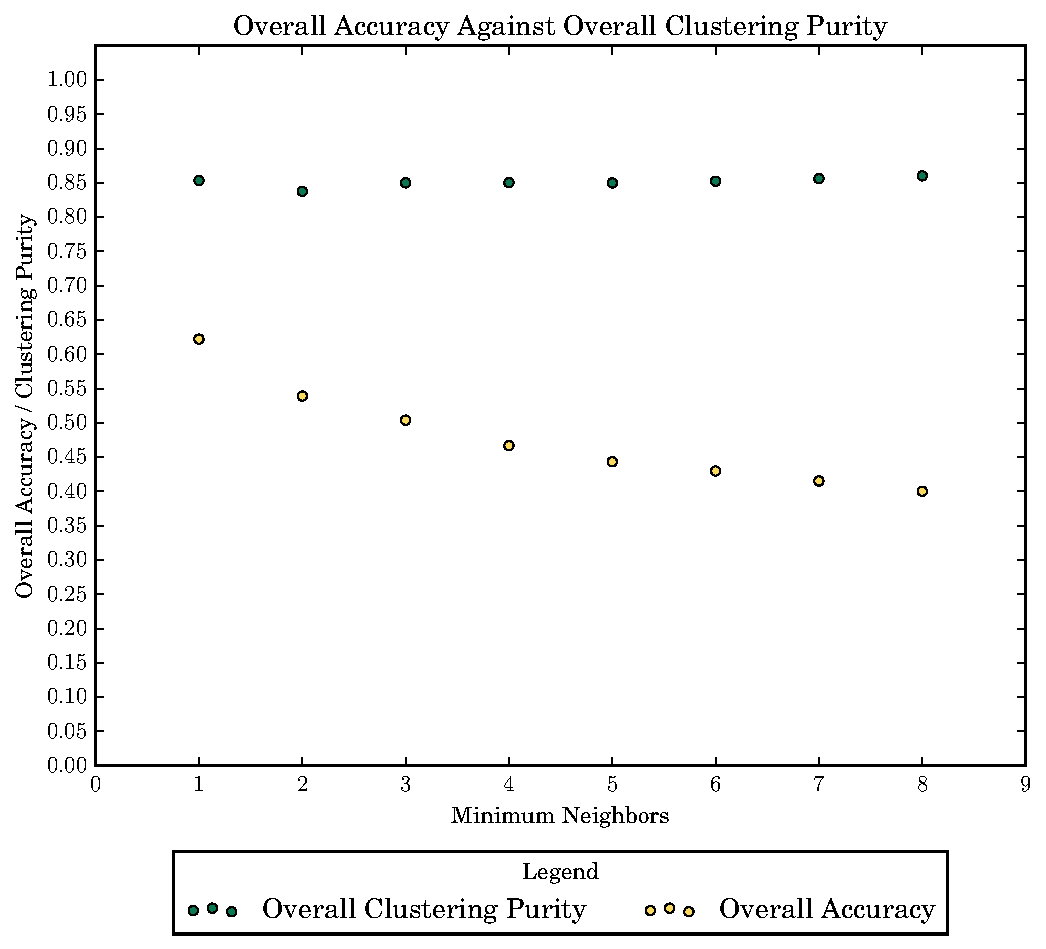
\includegraphics[width=\linewidth]{figures/bs/neigh_clust_accuracy.pdf}
    \caption{The overall accuracy decreases as we restrict  \minneigh{}. 
    The overall clustering purity stays relatively the same as we increase the value for \minneigh{}. 
    That is, for clustered \isols{}, the classification algorithm stays relatively the same relative to the number of isolates accurately clustered.}
    \label{fig:overall}
\end{figure}

Overall clustering purity, defined in \eqref{eq:overall_clustering}, is the number of \isols{} clustered that end up in a cluster where their \spec{} is the most plural \spec{}. 
The overall accuracy is the proportion of correctly classified \isols{} out of all the \isols{} under consideration.
We want to maximize both values, but would prefer the former over the latter.
Coverage is an issue we are concerned about, but we plan to mitigate this issue by leveraging  \cite{DBLP:conf/bibm/McGovernDKBVG15} against clusters of \isols{}.
%Using \cite{DBLP:conf/bibm/McGovernDKBVG15}, we can simplify the number of comparisons needed by comparing to clusters of \isols{} instead of \isols{} themselves.

\autoref{fig:overall} shows the overall accuracy compared to the overall clustering purity. 
A \minneigh{} value equal to 3 is the last \minneigh{} value where the overall accuracy stays above 0.50.
It is not for a lack of correctness, as \autoref{fig:clustered} shows, but more that \isols{} simply are not being clustered as we restrict the \minneigh{} value.
In fact, the overall clustering purity in \autoref{fig:overall} stays relatively constant.
This means that if an \isol{} is clustered by our algorithm, it will likely be clustered with other \isols{} of the same \spec{}.

% STRAINS --------------------
\subsection{Discussion}\label{sec:results:discussion}

In general, we observe two trends in our data. For the \isols{} that get clustered into strains,
our approach correctly identifies the \spec{} with over 80-85\% accuracy. This accuracy
is sufficient to conduct sophisticated \mst{} studies. Most of the strains discovered 
in the \cplop{} data show high degree of purity, and even considering the presence of 
a few large impure clusters, most of the clustered \isols{} fall into strains of high purity.


At the same time, the pure strain-based approach suffers from a drop in the coverage as the size of a cluster grows. 
This means that in general \cplop{} \isols{} tend to be very diverse
and come from strains for which not enough DNA material has been collected and pyrosequenced.
Identifying the \spec{} for \isols{} that do not fall into strains/clusters using the pure strain-based
method is impossible. In future work, our goal is to combine the \kNN{}-based \mst{} method
of \cite{DBLP:conf/bibm/McGovernDKBVG15} with the strain-based approach discussed in this paper
to increase coverage while preserving the high \mst{} accuracy.




%%%%%%%


%Considering how many \isols{} end up in clusters of high purity, as \autoref{fig:clust_purity_dist_3} shows, this occurrence appears to be infrequent.
%Nevertheless, viewing the progression of graphs in \autoref{fig:clust_pure} implies that the clusters morph and change into each other as we increase \minneigh{}.

One factor explaining the large impure clusters is the possibility that these
clusters represent what the  biologists call  ``transient'' strains, i.e., strains that 
persist in more than one \spec{}. 
%That is, certain strains might show up in many \spec{} and not just relegated to one \spec{}.
Such a characteristic can compound \mst{} by making certain strains of \ecoli{} less reliable as \fib{} for identifying \spec{}.
In \autoref{fig:clust_purity_dist}, we see evidence of that and it is revealed in \autoref{fig:clust_pure}.
One mitigation strategy may be to reduce the presence of these strains in library holding the \fib{}.
Another may be to fall back to an alternative \mst{} technique that works with \cplop{} when an unknown \isol{} falls into an impure cluster.  Finally, if a true transient strain is indeed
discovered, and an \isol{} is mapped to it, our \mst{} procedure can simply acknowledge the
that the query \isol{} belongs to a transient strain and provide information about the \spec{}
that show high frequency of \ecoli{} incidence from this strain.



%It also is possible that a more complicated or biologically-motivated strategy may work best.
%One avenue of validation we chose not to pursue was $k$-fold cross-validation.
%Previous work \cite{DBLP:conf/bibm/McGovernDKBVG15} has used it for validation.
%Future work may include it, but large $k$ values are likely to partition the dataset into groups different enough to create widely varying clusterings.